\documentclass[11pt]{article}
\usepackage[textwidth=18.0cm, textheight=23.0cm, top=2.0cm]{geometry}
\usepackage{pst-all}
\usepackage{amssymb}
\usepackage{tikz}
\usepackage{underscore}\begin{document}
\pagestyle{empty}


ClassName: \underline{\textbf{Class_10.2bp-32}}
\par
BinSize: \underline{\textbf{100 × 100}}
\par
ReduceSize: \underline{\textbf{100 × 100}}
\par
TypeNum: \underline{\textbf{80}}
\par
Num: \underline{\textbf{80}}
\par
OutS: \underline{\textbf{110000}}
\par
InS: \underline{\textbf{101043}}
\par
Rate: \underline{\textbf{0.919}}
\par
UB: \underline{\textbf{11}}
\par
LB0: \underline{\textbf{11}}
\par
LB: \underline{\textbf{11}}
\par
LBWithCut: \underline{\textbf{11}}
\par
NodeCut: \underline{\textbf{0}}
\par
ExtendedNodeCnt: \underline{\textbf{1}}
\par
GenNodeCnt: \underline{\textbf{1}}
\par
PrimalNode: \underline{\textbf{0}}
\par
ColumnCount: \underline{\textbf{11}}
\par
TotalCutCount: \underline{\textbf{0}}
\par
RootCutCount: \underline{\textbf{0}}
\par
LPSolverCnt: \underline{\textbf{1}}
\par
PricingSolverCnt: \underline{\textbf{0}}
\par
BranchAndBoundNum: \underline{\textbf{1}}
\par
isOpt: \underline{\textbf{true}}
\par
TimeOnPrimal: \underline{\textbf{0.000 s}}
\par
TimeOnPricing: \underline{\textbf{0.000 s}}
\par
TimeOnRmp: \underline{\textbf{0.078 s}}
\par
TotalTime: \underline{\textbf{0.140 s}}
\par
\newpage


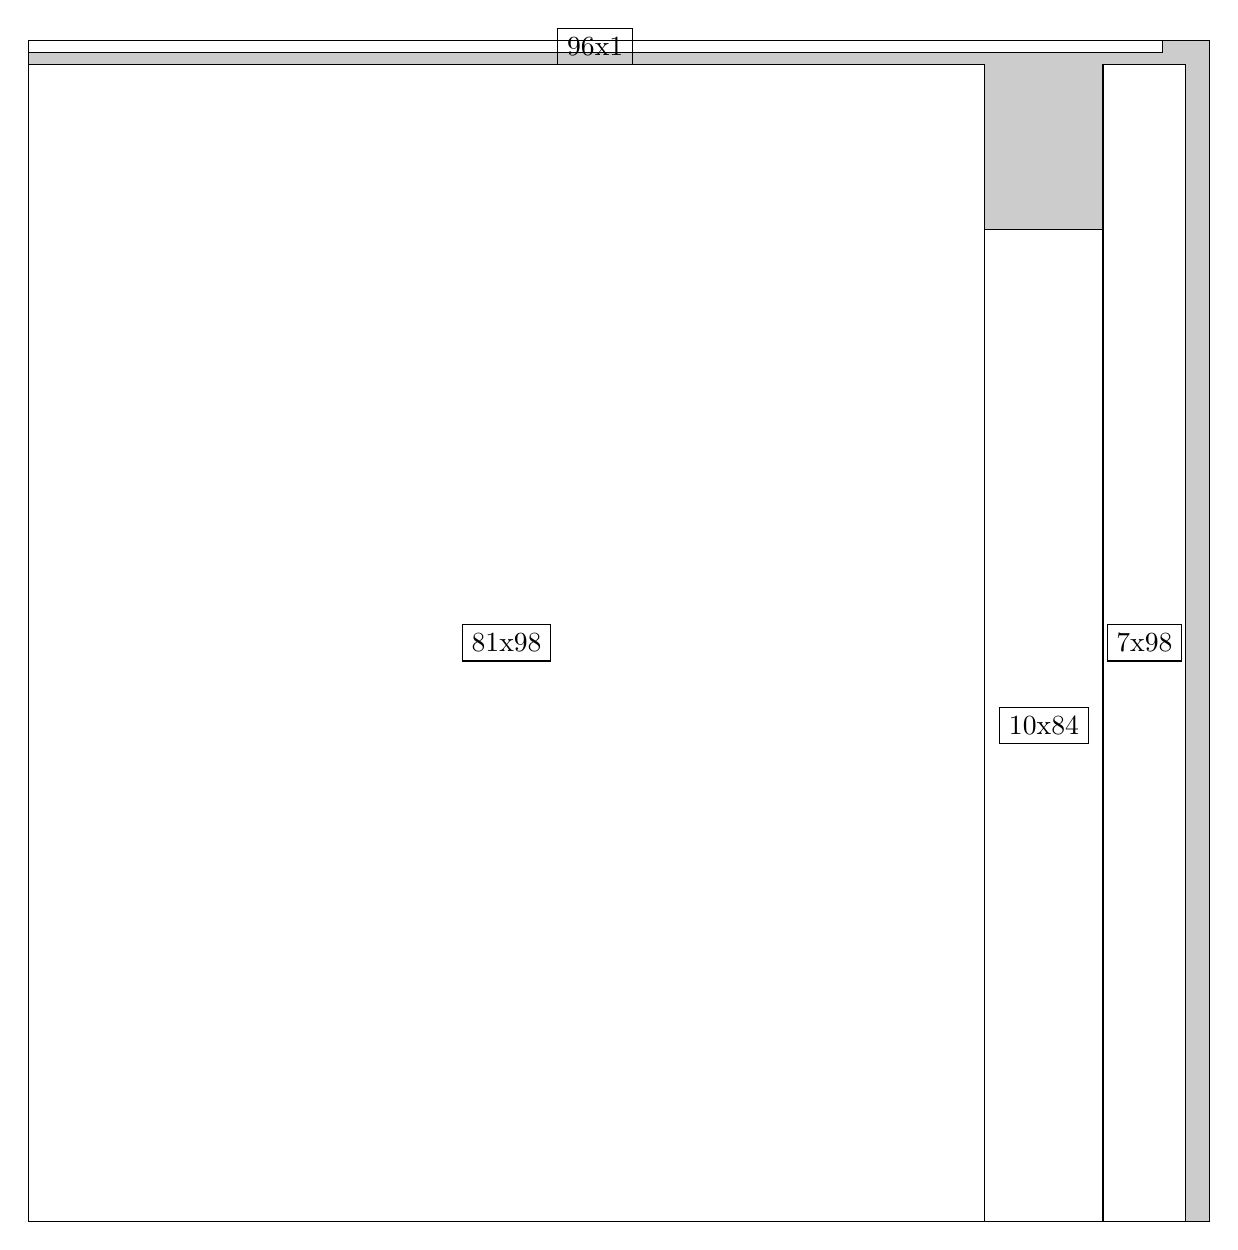
\begin{tikzpicture}[shorten >=1pt,scale=1.0,every node/.style={scale=1.0},->]
\tikzstyle{vertex}=[circle,fill=black!25,minimum size=14pt,inner sep=0pt]
\filldraw[fill=gray!40!white, draw=black] (0,0) rectangle (15.0,15.0);
\foreach \name/\x/\y/\w/\h in {81x98/0.0/0.0/12.15/14.7,10x84/12.15/0.0/1.5/12.6,7x98/13.65/0.0/1.05/14.7,96x1/0.0/14.85/14.399999999999999/0.15}
\filldraw[fill=white!40!white, draw=black] (\x,\y) rectangle node[draw] (\name) {\name} ++(\w,\h);
\end{tikzpicture}


w =81 , h =98 , x =0 , y =0 , v =7938
\par
w =10 , h =84 , x =81 , y =0 , v =840
\par
w =7 , h =98 , x =91 , y =0 , v =686
\par
w =96 , h =1 , x =0 , y =99 , v =96
\par
\newpage


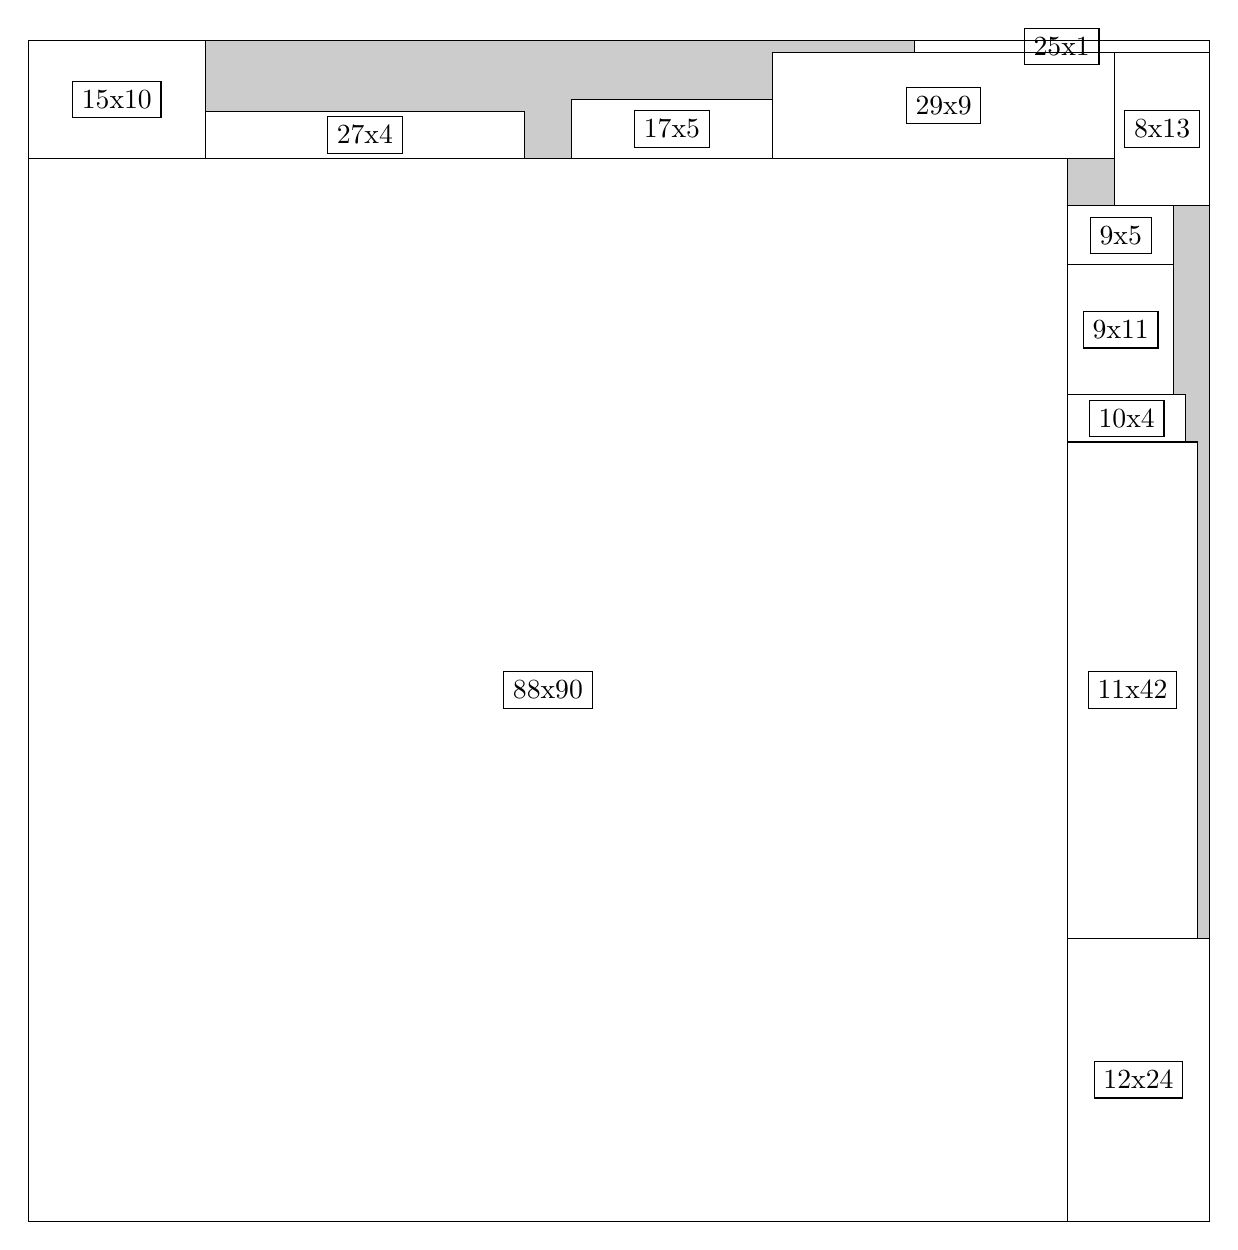
\begin{tikzpicture}[shorten >=1pt,scale=1.0,every node/.style={scale=1.0},->]
\tikzstyle{vertex}=[circle,fill=black!25,minimum size=14pt,inner sep=0pt]
\filldraw[fill=gray!40!white, draw=black] (0,0) rectangle (15.0,15.0);
\foreach \name/\x/\y/\w/\h in {88x90/0.0/0.0/13.2/13.5,11x42/13.2/3.5999999999999996/1.65/6.3,12x24/13.2/0.0/1.7999999999999998/3.5999999999999996,29x9/9.45/13.5/4.35/1.3499999999999999,15x10/0.0/13.5/2.25/1.5,27x4/2.25/13.5/4.05/0.6,8x13/13.799999999999999/12.9/1.2/1.95,9x11/13.2/10.5/1.3499999999999999/1.65,17x5/6.8999999999999995/13.5/2.55/0.75,9x5/13.2/12.15/1.3499999999999999/0.75,10x4/13.2/9.9/1.5/0.6,25x1/11.25/14.85/3.75/0.15}
\filldraw[fill=white!40!white, draw=black] (\x,\y) rectangle node[draw] (\name) {\name} ++(\w,\h);
\end{tikzpicture}


w =88 , h =90 , x =0 , y =0 , v =7920
\par
w =11 , h =42 , x =88 , y =24 , v =462
\par
w =12 , h =24 , x =88 , y =0 , v =288
\par
w =29 , h =9 , x =63 , y =90 , v =261
\par
w =15 , h =10 , x =0 , y =90 , v =150
\par
w =27 , h =4 , x =15 , y =90 , v =108
\par
w =8 , h =13 , x =92 , y =86 , v =104
\par
w =9 , h =11 , x =88 , y =70 , v =99
\par
w =17 , h =5 , x =46 , y =90 , v =85
\par
w =9 , h =5 , x =88 , y =81 , v =45
\par
w =10 , h =4 , x =88 , y =66 , v =40
\par
w =25 , h =1 , x =75 , y =99 , v =25
\par
\newpage


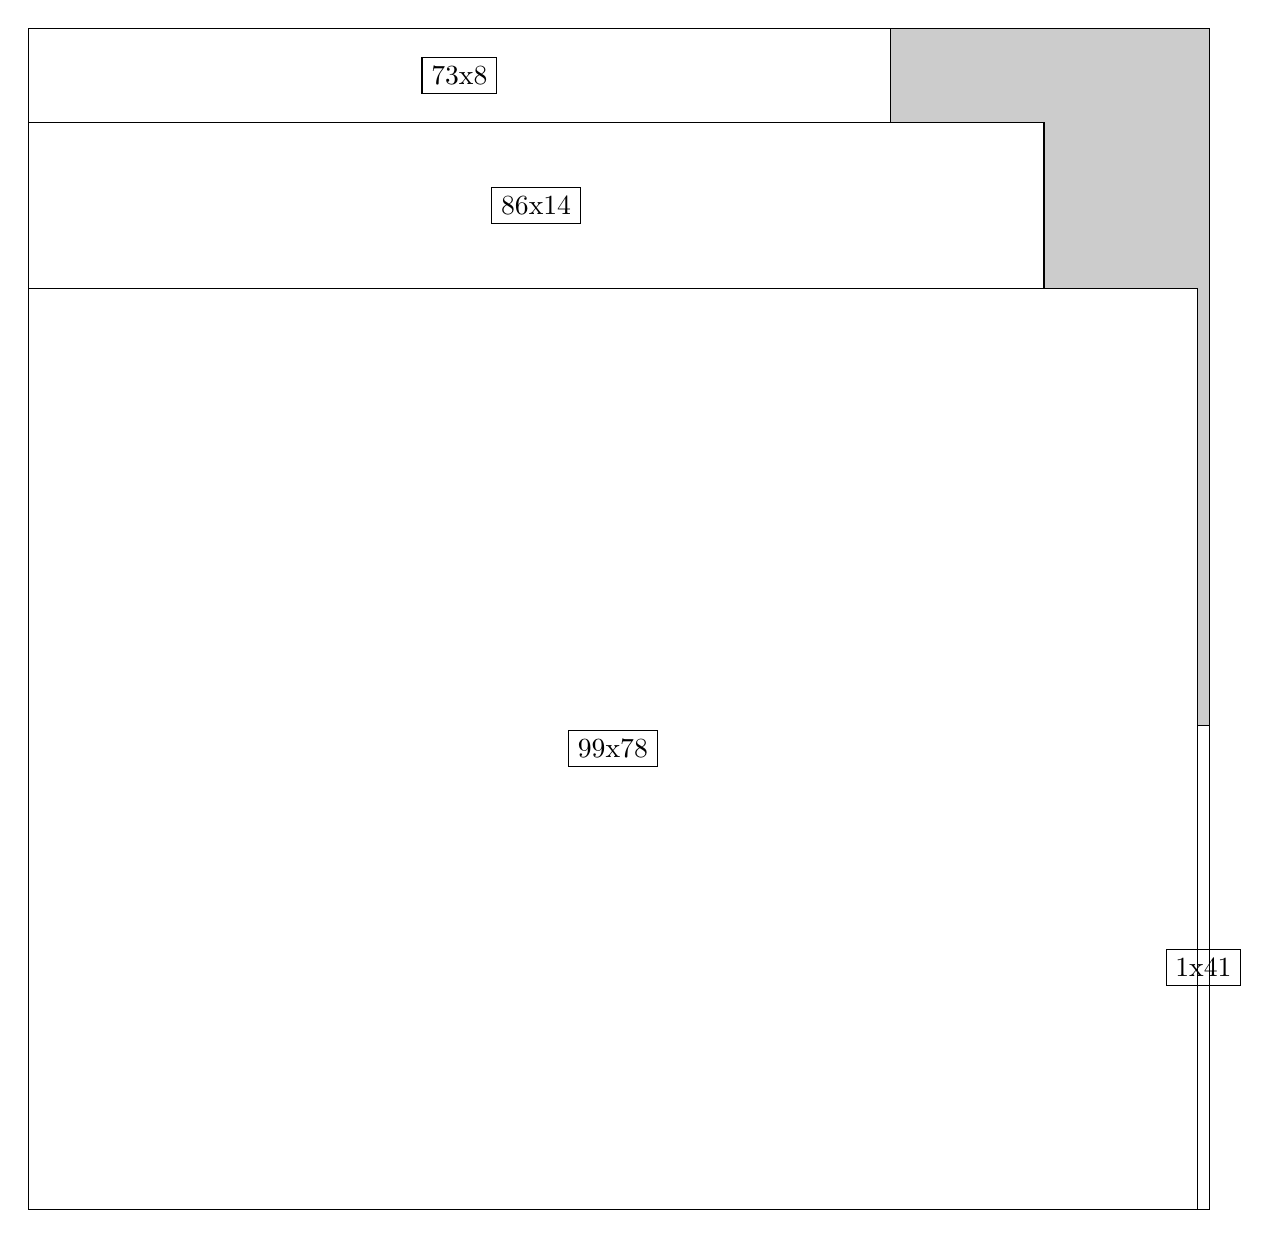
\begin{tikzpicture}[shorten >=1pt,scale=1.0,every node/.style={scale=1.0},->]
\tikzstyle{vertex}=[circle,fill=black!25,minimum size=14pt,inner sep=0pt]
\filldraw[fill=gray!40!white, draw=black] (0,0) rectangle (15.0,15.0);
\foreach \name/\x/\y/\w/\h in {99x78/0.0/0.0/14.85/11.7,86x14/0.0/11.7/12.9/2.1,73x8/0.0/13.799999999999999/10.95/1.2,1x41/14.85/0.0/0.15/6.1499999999999995}
\filldraw[fill=white!40!white, draw=black] (\x,\y) rectangle node[draw] (\name) {\name} ++(\w,\h);
\end{tikzpicture}


w =99 , h =78 , x =0 , y =0 , v =7722
\par
w =86 , h =14 , x =0 , y =78 , v =1204
\par
w =73 , h =8 , x =0 , y =92 , v =584
\par
w =1 , h =41 , x =99 , y =0 , v =41
\par
\newpage


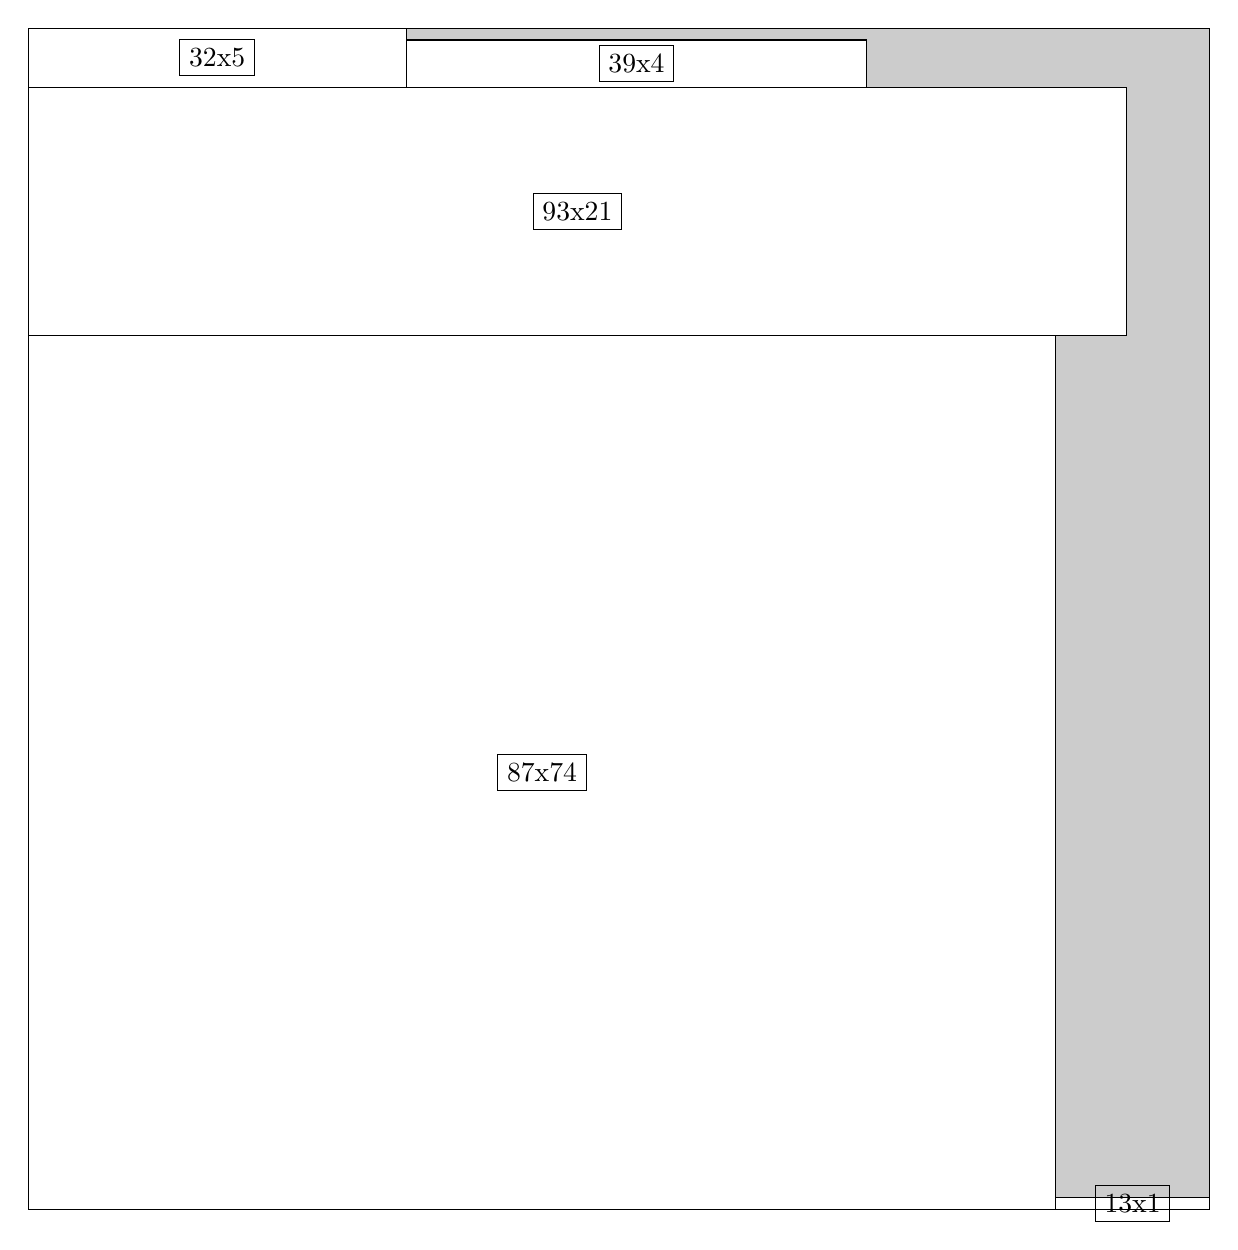
\begin{tikzpicture}[shorten >=1pt,scale=1.0,every node/.style={scale=1.0},->]
\tikzstyle{vertex}=[circle,fill=black!25,minimum size=14pt,inner sep=0pt]
\filldraw[fill=gray!40!white, draw=black] (0,0) rectangle (15.0,15.0);
\foreach \name/\x/\y/\w/\h in {87x74/0.0/0.0/13.049999999999999/11.1,93x21/0.0/11.1/13.95/3.15,32x5/0.0/14.25/4.8/0.75,39x4/4.8/14.25/5.85/0.6,13x1/13.049999999999999/0.0/1.95/0.15}
\filldraw[fill=white!40!white, draw=black] (\x,\y) rectangle node[draw] (\name) {\name} ++(\w,\h);
\end{tikzpicture}


w =87 , h =74 , x =0 , y =0 , v =6438
\par
w =93 , h =21 , x =0 , y =74 , v =1953
\par
w =32 , h =5 , x =0 , y =95 , v =160
\par
w =39 , h =4 , x =32 , y =95 , v =156
\par
w =13 , h =1 , x =87 , y =0 , v =13
\par
\newpage


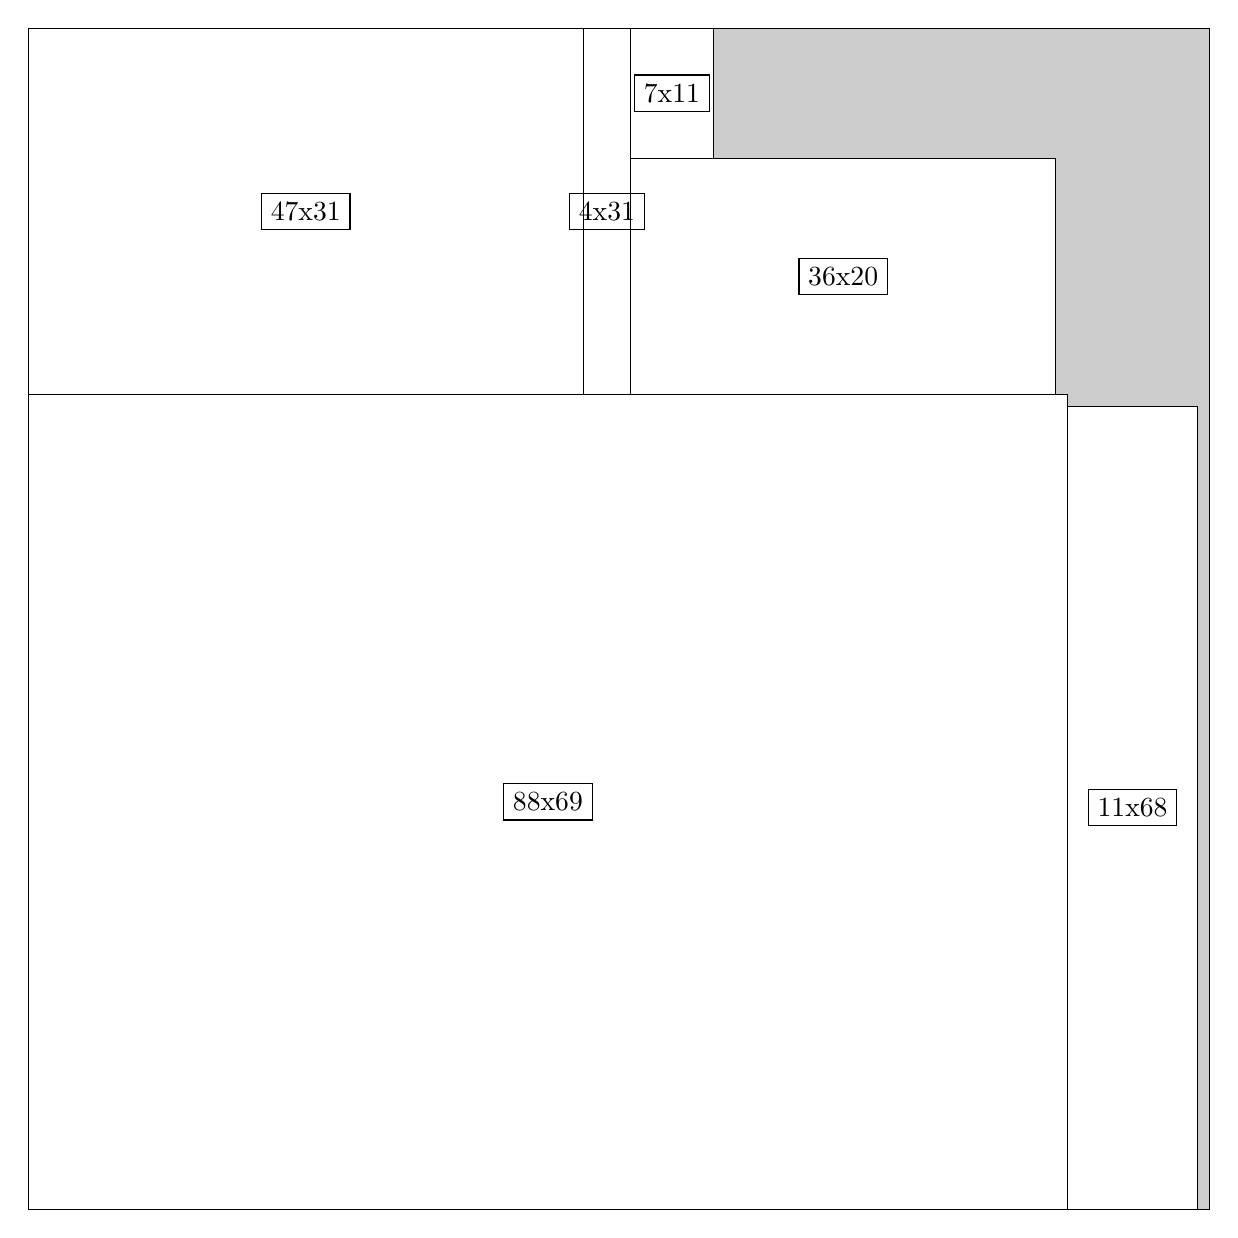
\begin{tikzpicture}[shorten >=1pt,scale=1.0,every node/.style={scale=1.0},->]
\tikzstyle{vertex}=[circle,fill=black!25,minimum size=14pt,inner sep=0pt]
\filldraw[fill=gray!40!white, draw=black] (0,0) rectangle (15.0,15.0);
\foreach \name/\x/\y/\w/\h in {88x69/0.0/0.0/13.2/10.35,47x31/0.0/10.35/7.05/4.6499999999999995,11x68/13.2/0.0/1.65/10.2,36x20/7.6499999999999995/10.35/5.3999999999999995/3.0,4x31/7.05/10.35/0.6/4.6499999999999995,7x11/7.6499999999999995/13.35/1.05/1.65}
\filldraw[fill=white!40!white, draw=black] (\x,\y) rectangle node[draw] (\name) {\name} ++(\w,\h);
\end{tikzpicture}


w =88 , h =69 , x =0 , y =0 , v =6072
\par
w =47 , h =31 , x =0 , y =69 , v =1457
\par
w =11 , h =68 , x =88 , y =0 , v =748
\par
w =36 , h =20 , x =51 , y =69 , v =720
\par
w =4 , h =31 , x =47 , y =69 , v =124
\par
w =7 , h =11 , x =51 , y =89 , v =77
\par
\newpage


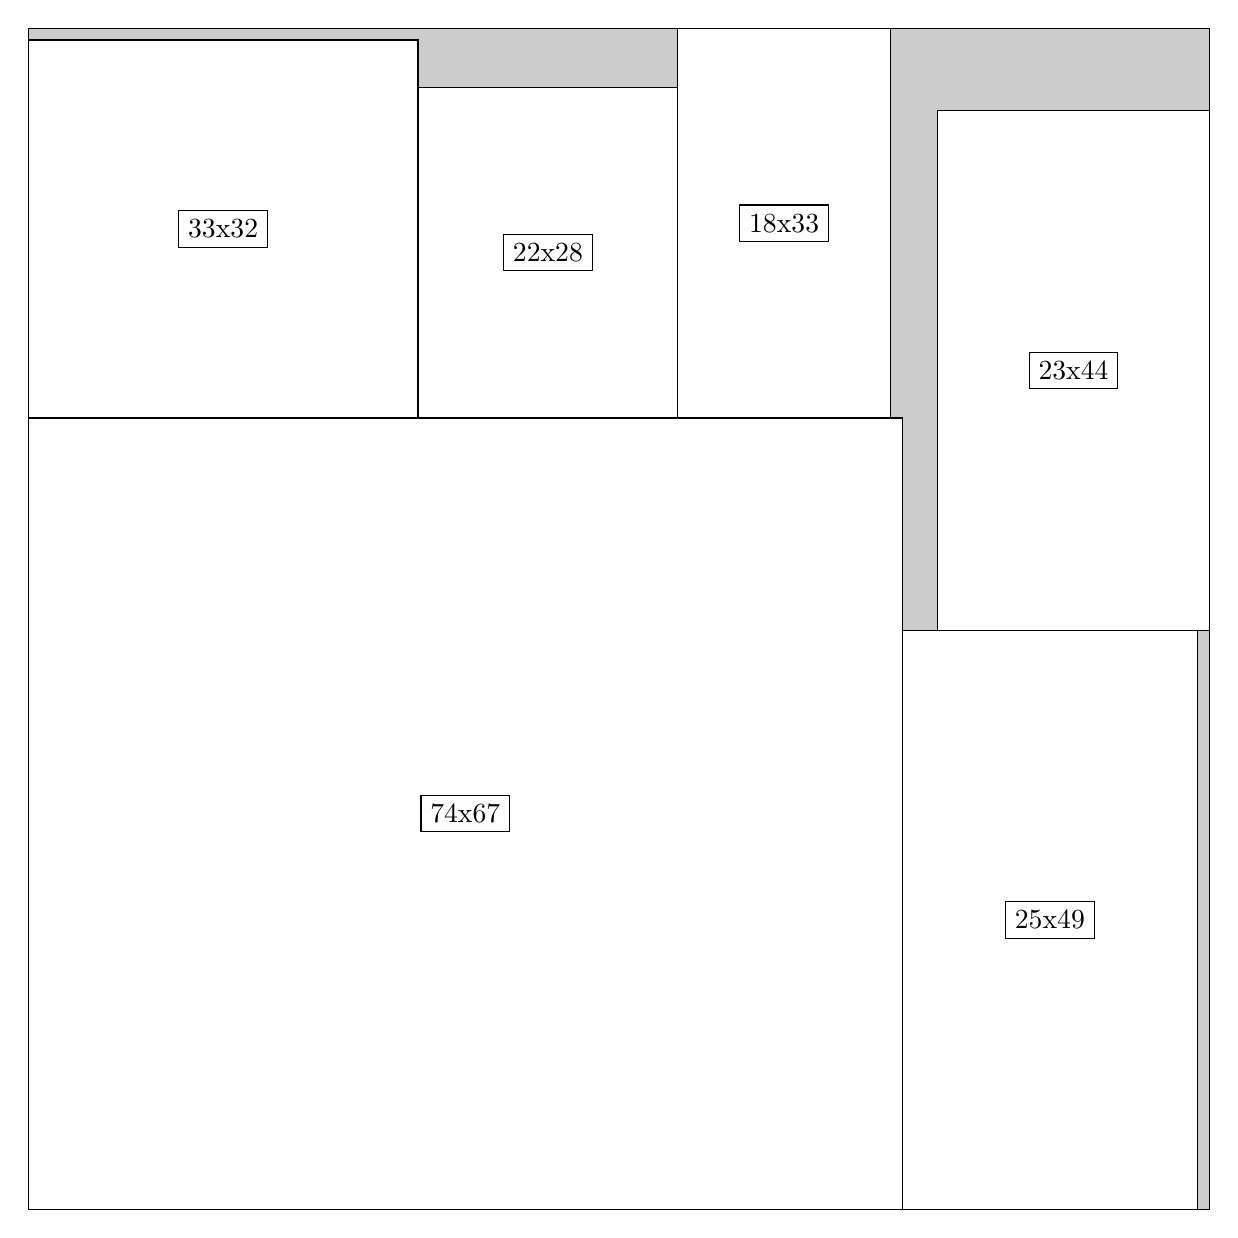
\begin{tikzpicture}[shorten >=1pt,scale=1.0,every node/.style={scale=1.0},->]
\tikzstyle{vertex}=[circle,fill=black!25,minimum size=14pt,inner sep=0pt]
\filldraw[fill=gray!40!white, draw=black] (0,0) rectangle (15.0,15.0);
\foreach \name/\x/\y/\w/\h in {74x67/0.0/0.0/11.1/10.049999999999999,25x49/11.1/0.0/3.75/7.35,33x32/0.0/10.049999999999999/4.95/4.8,23x44/11.549999999999999/7.35/3.4499999999999997/6.6,22x28/4.95/10.049999999999999/3.3/4.2,18x33/8.25/10.049999999999999/2.6999999999999997/4.95}
\filldraw[fill=white!40!white, draw=black] (\x,\y) rectangle node[draw] (\name) {\name} ++(\w,\h);
\end{tikzpicture}


w =74 , h =67 , x =0 , y =0 , v =4958
\par
w =25 , h =49 , x =74 , y =0 , v =1225
\par
w =33 , h =32 , x =0 , y =67 , v =1056
\par
w =23 , h =44 , x =77 , y =49 , v =1012
\par
w =22 , h =28 , x =33 , y =67 , v =616
\par
w =18 , h =33 , x =55 , y =67 , v =594
\par
\newpage


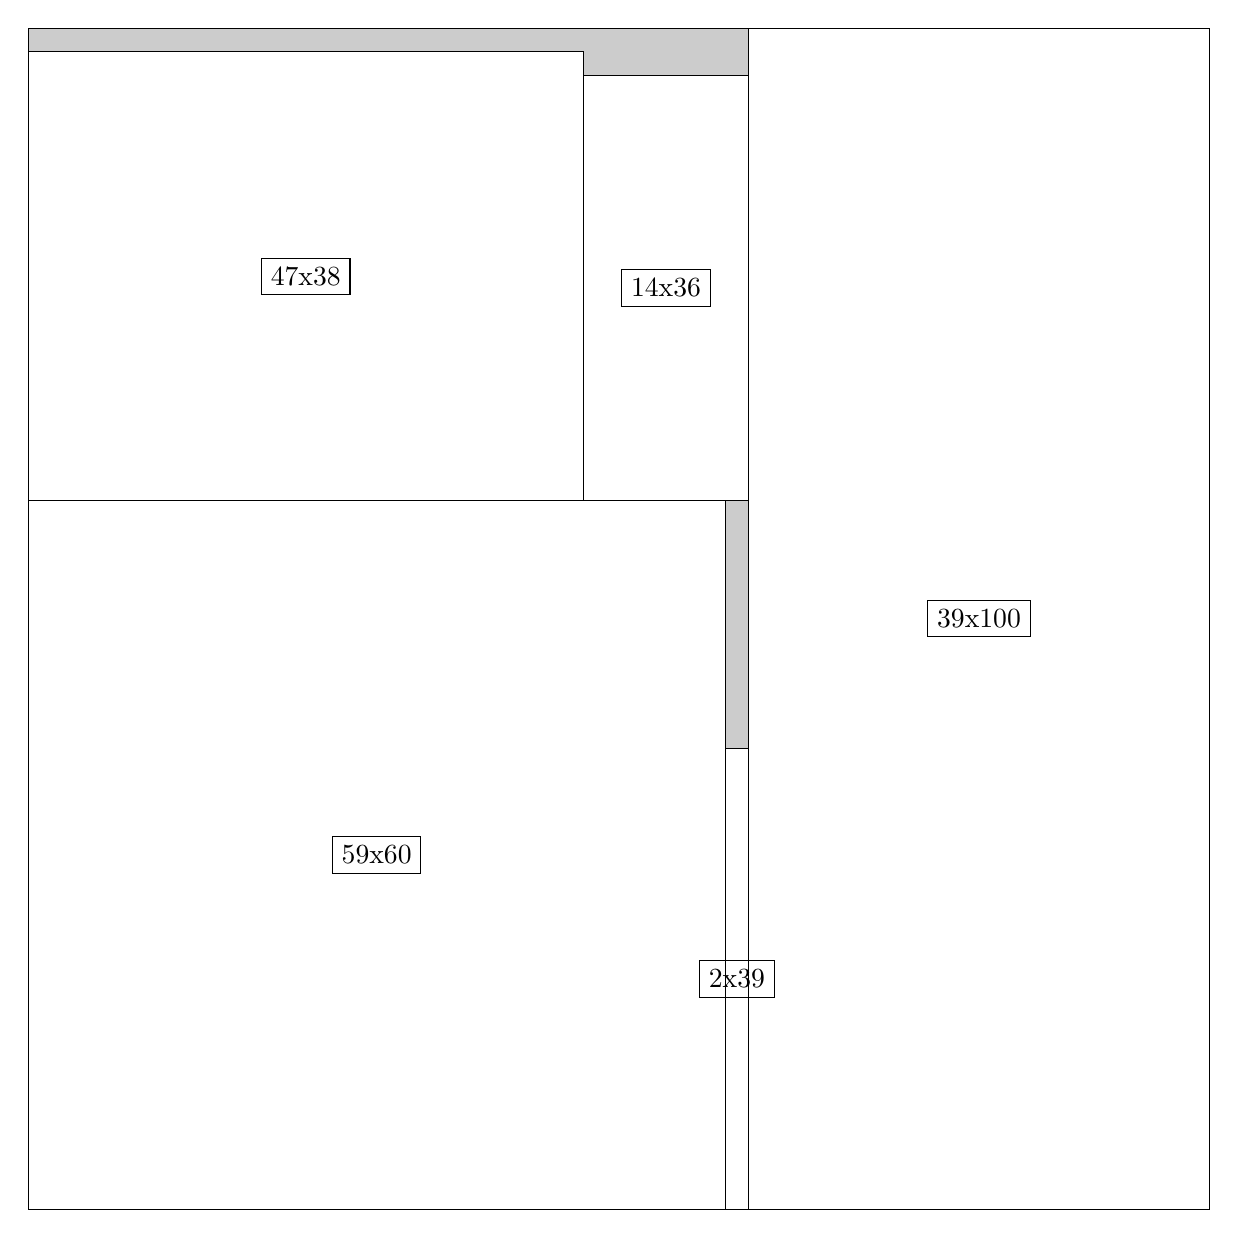
\begin{tikzpicture}[shorten >=1pt,scale=1.0,every node/.style={scale=1.0},->]
\tikzstyle{vertex}=[circle,fill=black!25,minimum size=14pt,inner sep=0pt]
\filldraw[fill=gray!40!white, draw=black] (0,0) rectangle (15.0,15.0);
\foreach \name/\x/\y/\w/\h in {39x100/9.15/0.0/5.85/15.0,59x60/0.0/0.0/8.85/9.0,47x38/0.0/9.0/7.05/5.7,14x36/7.05/9.0/2.1/5.3999999999999995,2x39/8.85/0.0/0.3/5.85}
\filldraw[fill=white!40!white, draw=black] (\x,\y) rectangle node[draw] (\name) {\name} ++(\w,\h);
\end{tikzpicture}


w =39 , h =100 , x =61 , y =0 , v =3900
\par
w =59 , h =60 , x =0 , y =0 , v =3540
\par
w =47 , h =38 , x =0 , y =60 , v =1786
\par
w =14 , h =36 , x =47 , y =60 , v =504
\par
w =2 , h =39 , x =59 , y =0 , v =78
\par
\newpage


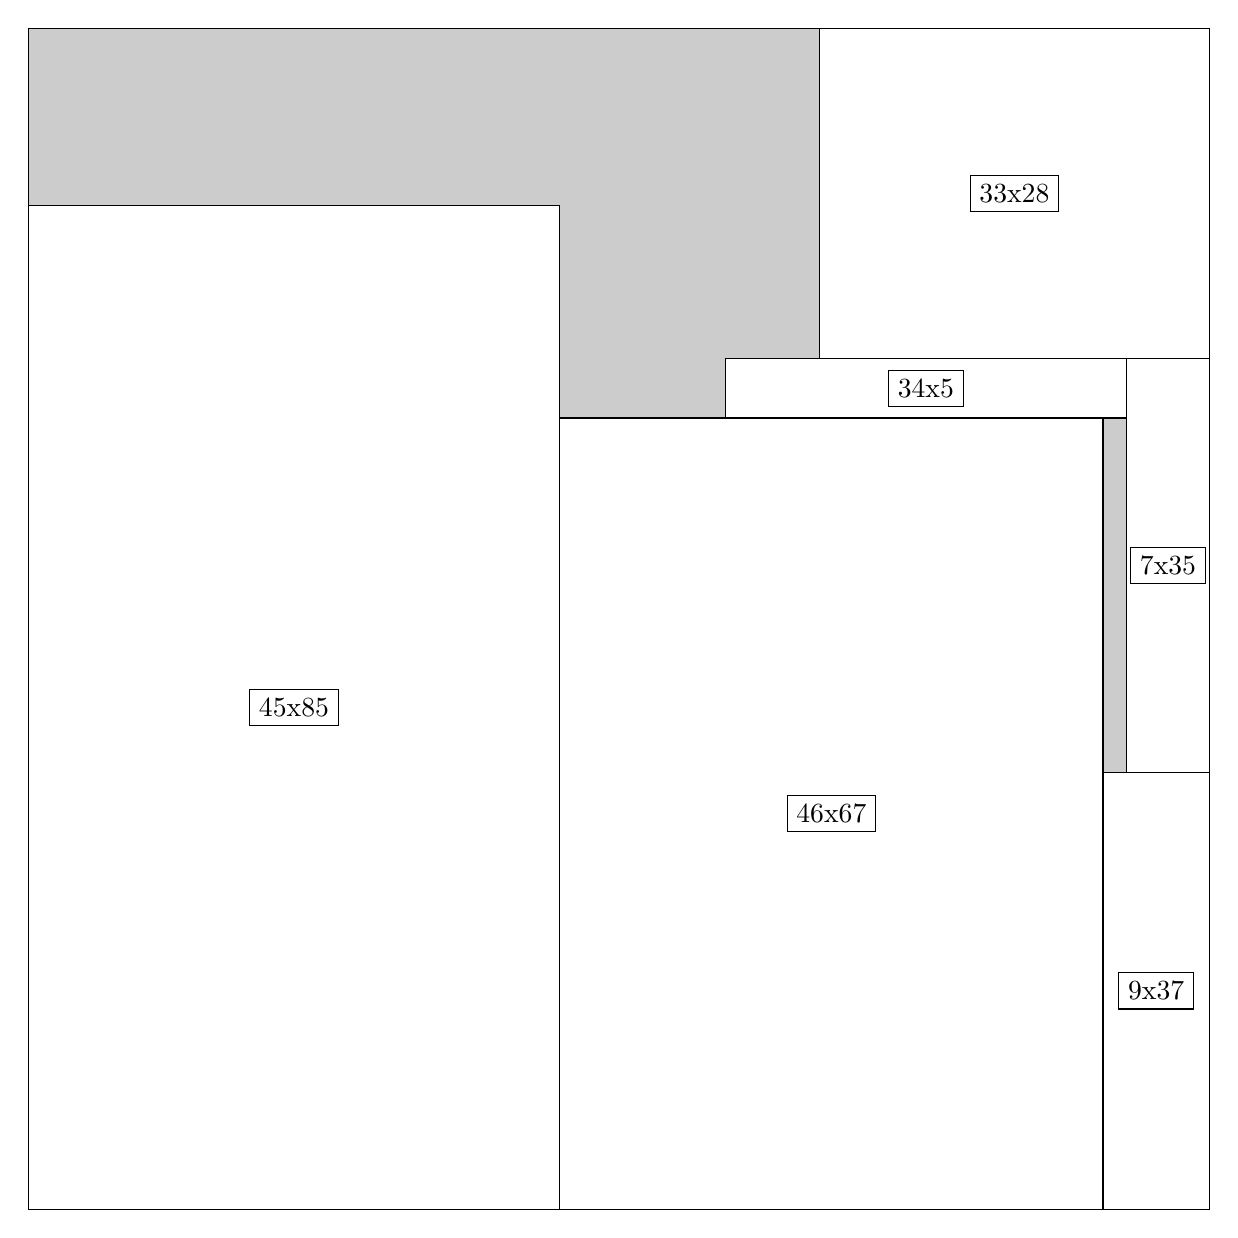
\begin{tikzpicture}[shorten >=1pt,scale=1.0,every node/.style={scale=1.0},->]
\tikzstyle{vertex}=[circle,fill=black!25,minimum size=14pt,inner sep=0pt]
\filldraw[fill=gray!40!white, draw=black] (0,0) rectangle (15.0,15.0);
\foreach \name/\x/\y/\w/\h in {45x85/0.0/0.0/6.75/12.75,46x67/6.75/0.0/6.8999999999999995/10.049999999999999,33x28/10.049999999999999/10.799999999999999/4.95/4.2,9x37/13.65/0.0/1.3499999999999999/5.55,7x35/13.95/5.55/1.05/5.25,34x5/8.85/10.049999999999999/5.1/0.75}
\filldraw[fill=white!40!white, draw=black] (\x,\y) rectangle node[draw] (\name) {\name} ++(\w,\h);
\end{tikzpicture}


w =45 , h =85 , x =0 , y =0 , v =3825
\par
w =46 , h =67 , x =45 , y =0 , v =3082
\par
w =33 , h =28 , x =67 , y =72 , v =924
\par
w =9 , h =37 , x =91 , y =0 , v =333
\par
w =7 , h =35 , x =93 , y =37 , v =245
\par
w =34 , h =5 , x =59 , y =67 , v =170
\par
\newpage


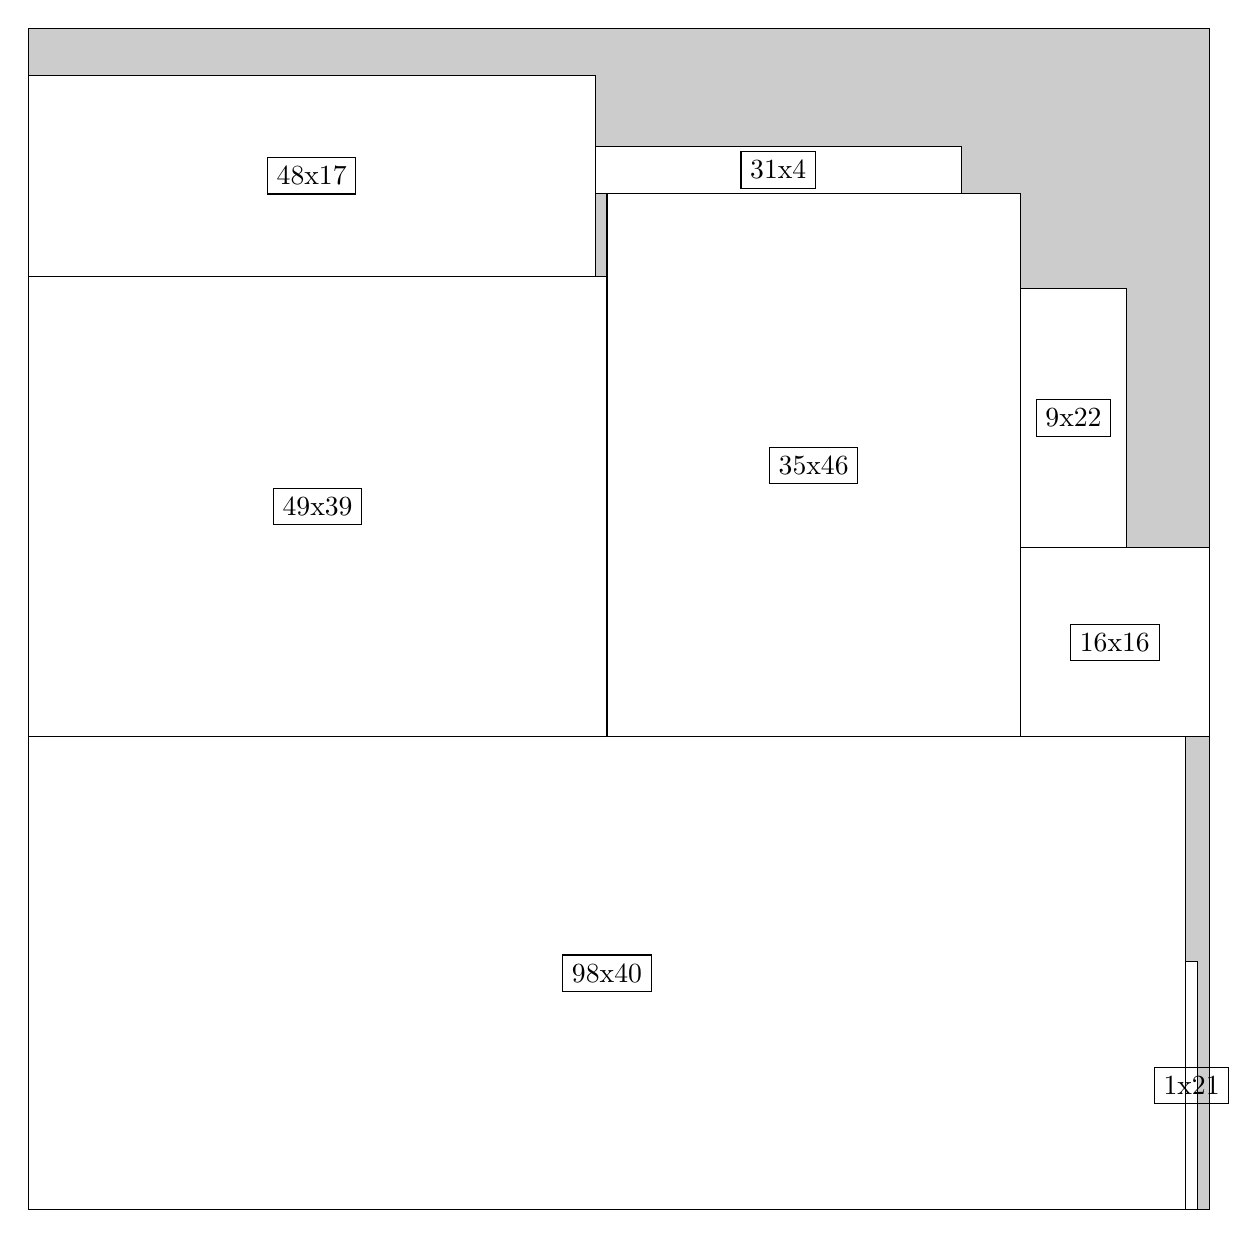
\begin{tikzpicture}[shorten >=1pt,scale=1.0,every node/.style={scale=1.0},->]
\tikzstyle{vertex}=[circle,fill=black!25,minimum size=14pt,inner sep=0pt]
\filldraw[fill=gray!40!white, draw=black] (0,0) rectangle (15.0,15.0);
\foreach \name/\x/\y/\w/\h in {98x40/0.0/0.0/14.7/6.0,49x39/0.0/6.0/7.35/5.85,35x46/7.35/6.0/5.25/6.8999999999999995,48x17/0.0/11.85/7.199999999999999/2.55,16x16/12.6/6.0/2.4/2.4,9x22/12.6/8.4/1.3499999999999999/3.3,31x4/7.199999999999999/12.9/4.6499999999999995/0.6,1x21/14.7/0.0/0.15/3.15}
\filldraw[fill=white!40!white, draw=black] (\x,\y) rectangle node[draw] (\name) {\name} ++(\w,\h);
\end{tikzpicture}


w =98 , h =40 , x =0 , y =0 , v =3920
\par
w =49 , h =39 , x =0 , y =40 , v =1911
\par
w =35 , h =46 , x =49 , y =40 , v =1610
\par
w =48 , h =17 , x =0 , y =79 , v =816
\par
w =16 , h =16 , x =84 , y =40 , v =256
\par
w =9 , h =22 , x =84 , y =56 , v =198
\par
w =31 , h =4 , x =48 , y =86 , v =124
\par
w =1 , h =21 , x =98 , y =0 , v =21
\par
\newpage


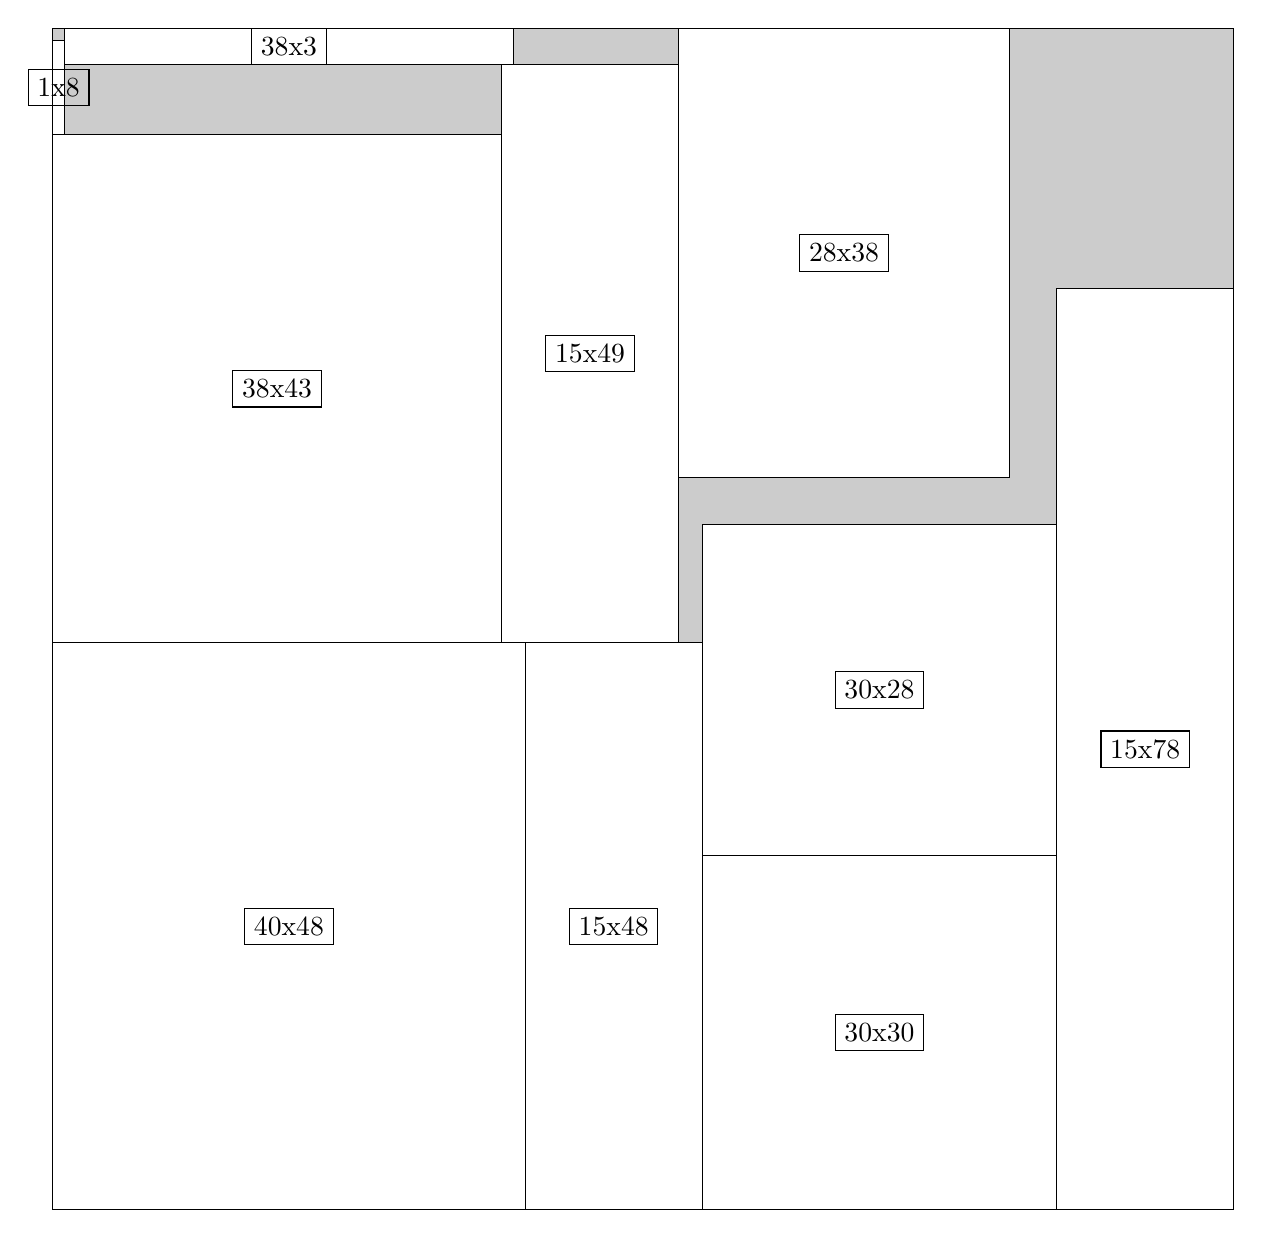
\begin{tikzpicture}[shorten >=1pt,scale=1.0,every node/.style={scale=1.0},->]
\tikzstyle{vertex}=[circle,fill=black!25,minimum size=14pt,inner sep=0pt]
\filldraw[fill=gray!40!white, draw=black] (0,0) rectangle (15.0,15.0);
\foreach \name/\x/\y/\w/\h in {40x48/0.0/0.0/6.0/7.199999999999999,38x43/0.0/7.199999999999999/5.7/6.45,15x78/12.75/0.0/2.25/11.7,28x38/7.949999999999999/9.299999999999999/4.2/5.7,30x30/8.25/0.0/4.5/4.5,30x28/8.25/4.5/4.5/4.2,15x49/5.7/7.199999999999999/2.25/7.35,15x48/6.0/0.0/2.25/7.199999999999999,38x3/0.15/14.549999999999999/5.7/0.44999999999999996,1x8/0.0/13.65/0.15/1.2}
\filldraw[fill=white!40!white, draw=black] (\x,\y) rectangle node[draw] (\name) {\name} ++(\w,\h);
\end{tikzpicture}


w =40 , h =48 , x =0 , y =0 , v =1920
\par
w =38 , h =43 , x =0 , y =48 , v =1634
\par
w =15 , h =78 , x =85 , y =0 , v =1170
\par
w =28 , h =38 , x =53 , y =62 , v =1064
\par
w =30 , h =30 , x =55 , y =0 , v =900
\par
w =30 , h =28 , x =55 , y =30 , v =840
\par
w =15 , h =49 , x =38 , y =48 , v =735
\par
w =15 , h =48 , x =40 , y =0 , v =720
\par
w =38 , h =3 , x =1 , y =97 , v =114
\par
w =1 , h =8 , x =0 , y =91 , v =8
\par
\newpage


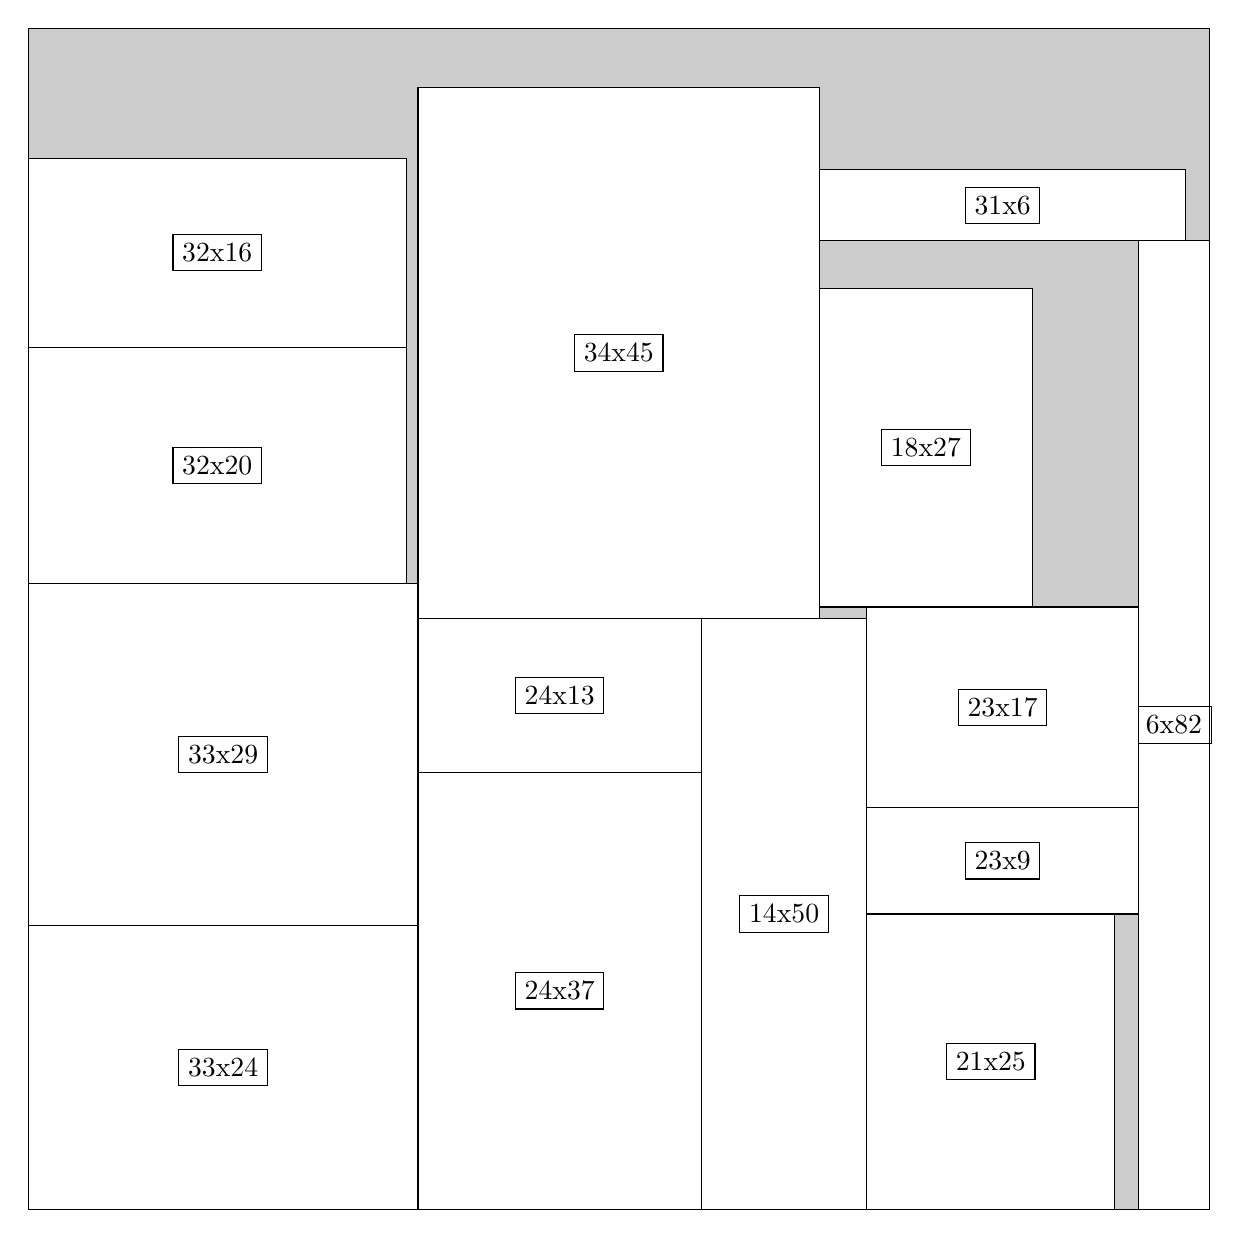
\begin{tikzpicture}[shorten >=1pt,scale=1.0,every node/.style={scale=1.0},->]
\tikzstyle{vertex}=[circle,fill=black!25,minimum size=14pt,inner sep=0pt]
\filldraw[fill=gray!40!white, draw=black] (0,0) rectangle (15.0,15.0);
\foreach \name/\x/\y/\w/\h in {33x24/0.0/0.0/4.95/3.5999999999999996,33x29/0.0/3.5999999999999996/4.95/4.35,24x37/4.95/0.0/3.5999999999999996/5.55,34x45/4.95/7.5/5.1/6.75,14x50/8.549999999999999/0.0/2.1/7.5,32x20/0.0/7.949999999999999/4.8/3.0,21x25/10.65/0.0/3.15/3.75,32x16/0.0/10.95/4.8/2.4,6x82/14.1/0.0/0.8999999999999999/12.299999999999999,18x27/10.049999999999999/7.6499999999999995/2.6999999999999997/4.05,23x17/10.65/5.1/3.4499999999999997/2.55,24x13/4.95/5.55/3.5999999999999996/1.95,23x9/10.65/3.75/3.4499999999999997/1.3499999999999999,31x6/10.049999999999999/12.299999999999999/4.6499999999999995/0.8999999999999999}
\filldraw[fill=white!40!white, draw=black] (\x,\y) rectangle node[draw] (\name) {\name} ++(\w,\h);
\end{tikzpicture}


w =33 , h =24 , x =0 , y =0 , v =792
\par
w =33 , h =29 , x =0 , y =24 , v =957
\par
w =24 , h =37 , x =33 , y =0 , v =888
\par
w =34 , h =45 , x =33 , y =50 , v =1530
\par
w =14 , h =50 , x =57 , y =0 , v =700
\par
w =32 , h =20 , x =0 , y =53 , v =640
\par
w =21 , h =25 , x =71 , y =0 , v =525
\par
w =32 , h =16 , x =0 , y =73 , v =512
\par
w =6 , h =82 , x =94 , y =0 , v =492
\par
w =18 , h =27 , x =67 , y =51 , v =486
\par
w =23 , h =17 , x =71 , y =34 , v =391
\par
w =24 , h =13 , x =33 , y =37 , v =312
\par
w =23 , h =9 , x =71 , y =25 , v =207
\par
w =31 , h =6 , x =67 , y =82 , v =186
\par
\newpage


\end{document}